\section{Recap}
\label{sec:recap}

The decade from 2010 to 2020 saw remarkable progress in speech recognition and
related technology. Figure~\ref{fig:asr_timeline} is a timeline of some of the
major developments in the research, software, and application of speech
recognition over the previous decade. The decade saw the launch and spread of
phone-based voice assistants like Apple Siri. Far-field devices like Amazon
Alexa and Google Home were also released and proliferated.

These technologies were enabled in-part by the remarkable improvement in the
word error rates of automatic speech recognition. This in turn was due to the
rise of deep learning in automatic speech recognition. The key drivers of the
success of deep learning in speech recognition have been 1) the curation of
massive transcribed data sets, 2) the rapid rate of progress in graphics
processing units, and 3) the improvement in the learning algorithms and model
architectures.

Thanks to these ingredients, the word error rate of speech recognizers improved
consistently and substantially throughout the decade. On two of the most
commonly studied benchmarks, automatic speech recognition word error rates have
surpassed those of professional transcribers (see figure~\ref{fig:wers}).

This remarkable progress begs the question: what's left for the coming
decade to the year 2030? In the following, I attempt to answer this question.
But, before I begin, I'd first like to share some observations on the general
problem of predicting the future. These findings are inspired by the
mathematician (as well as computer scientist and electrical engineer) Richard
Hamming, who also happened to be particularly adept at forecasting the future
of computing.

\begin{figure*}
\centering
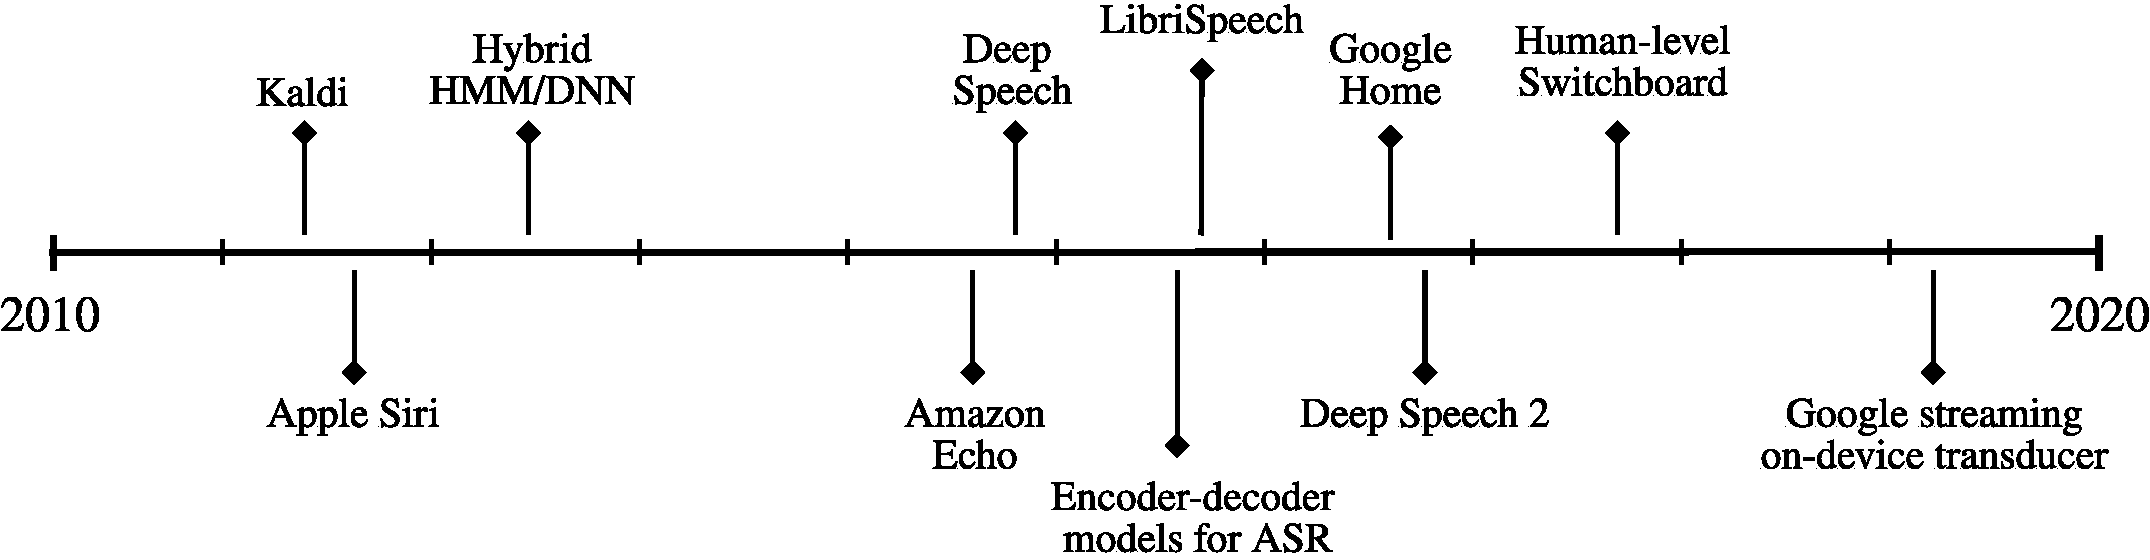
\includegraphics[width=\linewidth]{figures/asr_timeline}
\caption{A timeline of some of the major developments in speech recognition
    from the years 2010 to 2020. The decade saw the launch of
    voice-based devices and voice assistants, open-source and widely used
    speech recognition software like Kaldi~\citep{povey2011kaldi}, and larger
    benchmarks like LibriSpeech~\citep{panayotov2015librispeech}. We also saw
    speech recognition models improve starting from hybrid neural network
    architectures~\citep{hinton2012deep} to more end-to-end models including
    Deep Speech~\citep{hannun2014deep}, Deep Speech 2~\citep{amodei2016deep},
    encoder-decoder models with attention~\citep{chorowski2015attention}, and
    transducer-based speech recognition~\citep{he2019streaming}.}
\label{fig:asr_timeline}
\end{figure*}
